\documentclass[12pt]{article}
\usepackage[left=2cm, top=2cm, right=2cm, bottom=2cm]{geometry}
\usepackage[utf8]{inputenc}
\usepackage[T1]{fontenc}
\usepackage[french]{babel}
\usepackage{graphicx}
\usepackage{graphics}
\usepackage{amsmath}
\usepackage{tikz}
\usepackage{graphicx}
\usepackage{xcolor}
\usepackage{parskip}
\usepackage{physics}
\usepackage{tikz}


\title{\textbf{Méthodes expérimentales} \\ TP 4: Étude des propriétés thermodynamiques d'un gaz presque parfait}
\author{MENARD Alexandre \\ VIEILLEDENT Florent}

\setlength{\parindent}{1cm}

\begin{document}
\maketitle

\section*{Introduction}
Dans ce travail pratique, on cherchera à vérifier la loi des gaz parfaits. Le gaz utilisé sera l'air qu'on considère ici comme un gaz parfait. Dans un premier temps, on mesureras le pression d'un gaz en faisant varier le volume de ce gaz avec une température constante. On utiliseras pour cela une seringue et un pressiomètre Jeulin. 

On mesureras ensuite la pression d'un gaz à volume constant en faisant varier la température. On utilise pour ça une bouteille étanche et un manomètre. On utilise pour cela un gaz dans une seringue et un pressiomètre Jeulin. 





\newpage

\section{Relation entre le volume et la pression à température donnée}

Dans cette première expérience on cherche à vérifier que le produit PV est une constante. Pour cela, on calcule la pression d'un gaz pour différentes valeurs de volumes, sans changer la température. 	

\subsection{Expérimentation}

La seringue est placé initialement sur $15\, cm^3$. On relie ensuite la seringue au pressiomètre Jeulin gràce à un tuyau. On fait varier le volume de la seringue et on note la pression donnée par le pressiomètre. 

\begin{figure}[!h]
	\begin{center}
		\includegraphics[scale=0.3]{Schéma_seringue.png}
		\label{Schéma_seringue}
		\caption{Schéma de la première expérience avec la seringue et le pressiomètre}
	\end{center}
\end{figure}

[INSÉRER PHOTO PREMIÈRE EXPÉRIENCE]

On note $V_{seringue}$ le volume à l'intérieur de la seringue. On fait varier ce volume de $15\, cm^3$ à $60\, cm^3$ tout les $5\, cm^3$. La seringue est graduée tout les $cm^3$, donc notre incertitude sur le volume est $\delta V_{seringue}=0.5 \, cm^3$.  On note pour chaque volume la pression donnée par le pressiomètre. L'incertitude sur le pressiomètre est de $2\% $. On a donc $\delta P = 0.02*P$. On répète les mesures 3 fois pour avoir une meilleur estimation de l'incertitude. On note respectivement P1,P2 et P3 les mesures de pressions lors de la première, deuxième et troisième mesure. 

\newpage
\begin{table}[h!]
	\begin{center}
		\begin{tabular}{|r|r|r|r|r|r|r|}	
\hline
 $V_{seringue} (cm^3)$ &  P1 (hPa) &  $\delta P1(hPa)$ &  P2 (hPa) &  $\delta P2(hPa)$ &  P3 (hPa) &  $\delta P3(hPa)$ \\
\hline
            15 &              1003 &            20 &              1050 &            21 &              1070 &            21 \\
            20 &               792 &            16 &               810 &            16 &               816 &            16 \\
            25 &               640 &            13 &               654 &            13 &               652 &            13 \\
            30 &               542 &            11 &               552 &            11 &               556 &            11 \\
            35 &               468 &             9 &               474 &             9 &               480 &            10 \\
            40 &               410 &             8 &               417 &             8 &               427 &             9 \\
            45 &               368 &             7 &               374 &             7 &               374 &             7 \\
            50 &               331 &             7 &               337 &             7 &               338 &             7 \\
            55 &               302 &             6 &               304 &             6 &               308 &             6 \\
            60 &               276 &             6 &               283 &             6 &               284 &             6 \\
\hline
		\end{tabular}
	\end{center}
\end{table}

\newpage
\section{Relation entre la température et la pression à volume constant}
Dans cette expérience, on cherche à valider ou non la loi des gaz parfaits en variant la température et la pression
à volume constant. On en déduira également la valeur du "zéro absolu" à une pression nulle en extrapolant notre courbe.

\subsection{Théorie}
Ici, on a la pression $P$ et la température $T$ qui varient, et le volume $V$ constant. Ainsi, selon la loi des gaz parfaits:

\begin{equation}
    PV = nRT
\end{equation}

On obtient directement que le produit $V = \frac{nRT}{P}$ est constant. Pour vérifier nos mesures, nous avons donc plusieurs solutions:
\begin{itemize}
    \item Tracer le volume $V$ en fonction du produit $\frac{nRT}{P}$ en utilisant les valeurs de $T$ et $P$ que l'on mesure.
    On s'attendra donc à obtenir une droite d'équation $y = V$ pour que la loi des gazs parfait soit vérifiée. De plus, cette approche nous permettra de déterminer le volume réel
    que l'on a dans notre expérience, car dans la partie expérimentation, nous allons supposer un volume de 250mL, ce qui n'inclut pas le volume du tuyau et du manomètre.
    \item Tracer $P$ en fonction de $T$, car $P = \frac{nR}{V} T$, on doit donc obtenir une droite. Cette approche permet de déterminer la valeur de la température à $P=0Pa$.
\end{itemize}

\subsection{Expérimentation}
Maintenant que nous savons ce que l'on doit chercher, on passe à l'expérimentation. L'expérience consiste à
plonger une bouteille d'air de 250mL dans un bécher suffisament grand pour immerger la bouteille et de chauffer l'eau du bécher de 20°C à 60°C.
On relève ensuite la température de l'eau et la pression tous les degrés.

\begin{figure}[!h]
	\begin{center}
		\includegraphics[scale=0.05]{img/exp2.jpg}
		\label{Exp2}
		\caption{Montage de l'expérience}
	\end{center}
\end{figure}

\textbf{Remarque:} le thermocouple est plongé dans l'eau, et non l'air de la bouteille, pourtant, nous allons utiliser la pression de l'air dans
la bouteille, on a donc deux variables qui representent des systèmes différents car rien ne nous affirme qu'il y a thermalisation entre l'air de la bouteille et l'eau.
Pour s'en convaincre, à la fin de l'expérience, nous laisserons refroidir l'eau naturellement (donc très lentement) tout en prenant les valeurs de températures et pression. 
Le refroidissement long nous assure la condition de thermalisation entre nos deux systèmes. Ainsi, si lors du refroidissement, il y a recouvrement entre les valeurs pendant le chauffage et 
refroidissement, on pourra affirmer qu'il y avait thermalisation pendant le chauffage.

\begin{figure}[!h]
	\begin{center}
		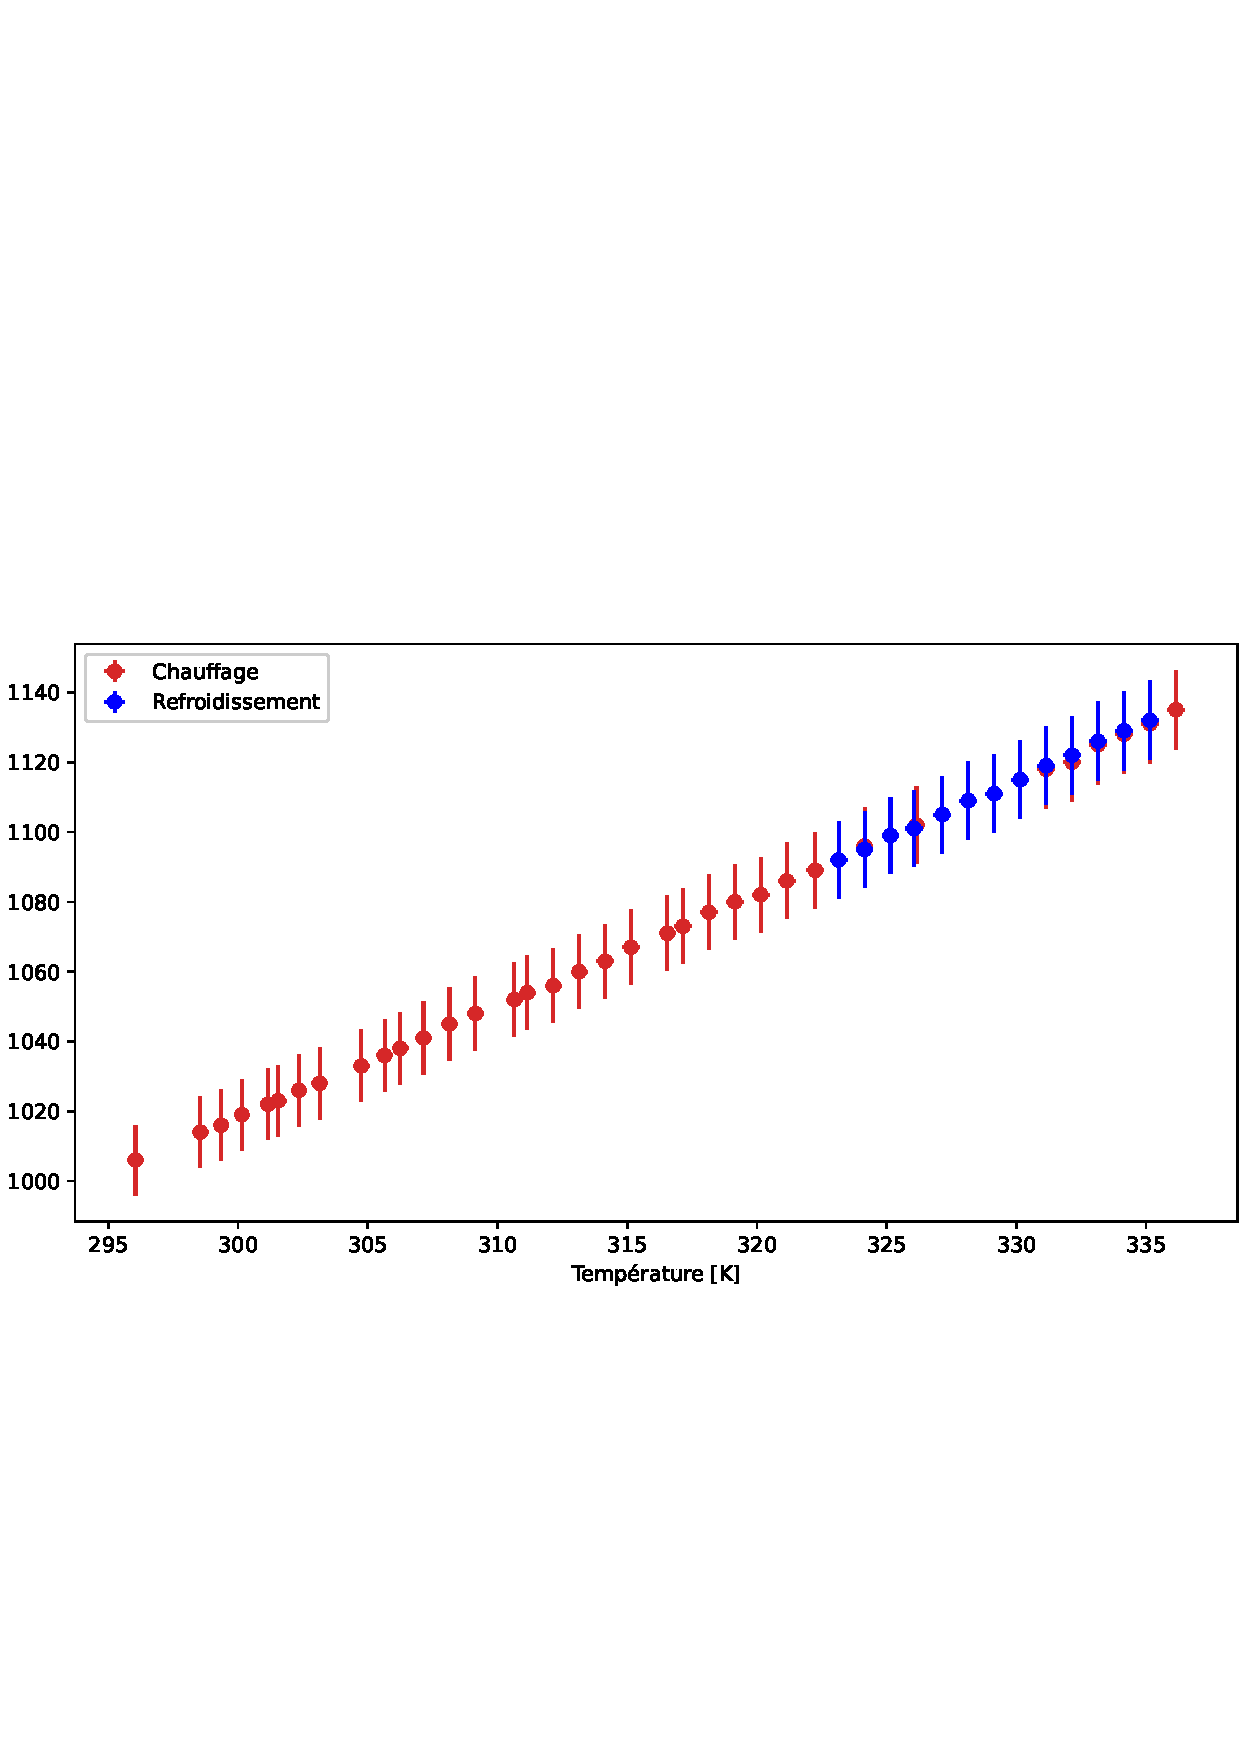
\includegraphics[scale=0.7]{img/exp2_graph1.png}
		\label{Exp2_graph1}
		\caption{Pression $P$ en fonction de la température}
	\end{center}
\end{figure}

\end{document}
